\chapter{Experiments}

\section{Datasets}
\label{sec:exp-datasets}

\subsection{MPII Human Pose}
\label{sec:exp-mpii}

In \cite{andriluka_2d_2014}, the authors present a dataset for 2D human pose estimation on still images.
It contains $25.000$ images, where $40.000$ persons were annotated.
The annotations include $16$ joint annotations in addition to an indicator of whether or not the joint is visible or not.
The $16$ joints are \textit{left / right ankle}, \textit{left / right knee}, \textit{left / right hip}, \textit{left / right elbow}, \textit{left / right shoulder}, \textit{left / right wrist}, \textit{pelvis}, \textit{thorax}, \textit{upper neck} and \textit{top of the head}.
See TODO for example images, including the pose annotations.
In addition, the body center coordinates are given in addition to a scale indicating the size of the person bounding box w.r.t. $200$ pixels.
Also, a bounding box of the head is given, which is used to compute the \textit{PCKh} metric (see \sref{sec:exp-pckh}).
The images were extracted from YouTube videos and do not contain artifacts commonly found in videos like compression or blur.
Additionally, each image is assigned an activity performed in the video it was extracted from, totalling $401$ total activities.
However, these annotations were not used for Human Action Recognition since they are too fine-grained and the number of samples per activity is too low for training a deep neural network.

We follow the approaches from \cite{luvizon_2d/3d_2018} for preprocessing, which the authors present in their supplemental material.
First, a person bounding box is estimated using the center body annotation from the dataset.
The authors multiply the scale given by the annotation $s_{orig}$ by $1.25$, resulting in $s_{new}$.
They do not motivate the reason for using this specific value, but it most likely was used to enlarge the bounding box to contain more context around the person.
Next, they compute the width and height using $s_{new} \cdot 200$, which results in a square bounding box.
In addition, the authors also alter the center position $(c_x,  c_y)$ given by the annotation by computing $(c_{x}^{new}, c_y^{new}) = (c_x, c_y + s_{new} \cdot 12)$.
Again, the authors do not provide a reasoning for moving the center position further towards the neck of the person in this way.
Once the bounding box is computed, the image is cropped to the size of the bounding box around the newly computed center coordinate.
In the case where a joint annotation falls outside of the now cropped image, the authors set the visibility of the joint to $0$ and set the $(x,y)$ coordinates of the joint to $(-1e9, -1e9)$.

Additionally, the authors introduce parameters used for augmentation.
These values are sampled from their respective sets whenever augmentation is performed.
Specifically, they introduce $s_{aug} \in \{0.7, 1, 1.3\}$ which gets multiplied with $s_{new}$ computed earlier.
Also, $r_{aug} \in \{-40, -35, \dots, 35, 40\}$ is introduced to rotate the image $r_{aug}$ degrees around its center, possibly introducing black borders around the image.
Moreover, when augmenting, the image is horizontally flipped with a chance of $50$ percent.
See TODO for multiple examples of different augmented images. 

The dataset does not contain annotations for the test data, other than the scale and center coordinates.
To evaluate the test images, the joints need to be evaluated and the results need to be send to the authors for comparison to the ground truth pose.
This ensures that the test data annotations are not mistakenly or maliciously used in training.
For all datasets used in the experiments, $10$ percent of the training datapoints were withheld from training and used as validation data.

\subsection{Penn Action}
\label{sec:exp-penn}

Another dataset used in \cite{luvizon_2d/3d_2018} is the Penn Action dataset \cite{zhang_actemes_2013}.
It contains $2326$ video clips of $15$ different actions performed.
The actions performed are mostly sports related and include \textit{baseball swing}, \textit{clean and jerk}, \textit{jumping jacks}, \textit{pushup}, \textit{strum guitar}, \textit{bench press}, \textit{golf swing}, \textit{baseball pitch}, \textit{situp}, \textit{tennis forehand}, \textit{bowling}, \textit{jump rope}, \textit{pullup}, \textit{squat} and \textit{tennis serve}.
In addition, the authors provide annotations for $13$ body joints,
including \textit{left and right shoulders, elbows, wrists, hips and knees} as well as one annotation of the \textit{head} of the person.
Some example images can be seen in TODO. 

It was decided by \cite{luvizon_2d/3d_2018} that the number of joints should be identical to the ones presented in \cite{andriluka_2d_2014} \sref{sec:exp-mpii} because the network assumes a fixed number of joints.
This then means that the network architecture does not need to be changed, no matter which dataset is used.
Specifically, the \textit{pose cube} dimensionality does not need to be changed.
To achieve this, the \textit{head} annotation of the Penn Action dataset is mapped to the \textit{upper neck} joint of the MPII dataset and the missing joints were interpreted as not visible.
The augmentation is identical to the augmentation mentioned in \sref{sec:exp-mpii}.

For some experiments, we compute a ground truth bounding box of the person by calculating the minimum and maximum $x$ and $y$ coordinates of the pose and defining these as the corners of the bounding box.
Additionally, to include more context, we decided to increase the bounding box by $30$ pixels in both dimensions.

Additionally, the authors in \cite{luvizon_2d/3d_2018} decide to process the video clips in chunks of $16$ frames.
This is again important since the network architecture can be kept the same because \textit{pose cube} dimensions do not change that way.
Thus, we decided to precompute $16$ frames subclips, which we call \textit{fragments}, and save them separately to increase the training speed, since the preprocessing and extraction of the subclips does not need to be done at training time. 

\subsection{JHMDB}
\label{sec:exp-jhmdb}

Similar to \cite{zhang_actemes_2013} \sref{sec:exp-penn}, the JHMDB dataset \cite{jhuang_towards_2013} contains annotations for pose and action in video clips.
The dataset was created by taking a subset of the HMDB action recogntion dataset \cite{kuehne_hmdb:_2011}, which was then annotated using the \textit{puppet tool} \cite{zuffi_pictorial_2012}.
This tool allows to not only annotate the pose of the person but also automatically computes a binary segmentation map of the person, further referred to as the \textit{puppet mask}.
See TODO for a visualization of the annotation process and the puppet tool.

The clips in the HMDB dataset were taken from YouTube.
The annotated subset contains the following actions:
\textit{brush hair}, \textit{catch}, \textit{clap}, \textit{climb stair}, \textit{golf}, \textit{jump}, \textit{kick ball}, \textit{pick}, \textit{pour}, \textit{pullup}, \textit{push}, \textit{run}, \textit{shoot ball}, \textit{shoot bow}, \textit{shoot gun}, \textit{sit}, \textit{stand}, \textit{swing baseball}, \textit{throw}, \textit{walk} as well as \textit{wave}.
Some example images of the dataset can be seen in TODO.
Notice that the actions are more diverse, in comparison to the Penn Action dataset, specifically because it also contains non-sport activities.

The puppet tool defines $15$ different joints.
They are identical to the ones annotated in the Penn Action dataset, but additionally contain \textit{neck} and \textit{belly}.
The same procedure was used to map the joints to the format provided by the MPII dataset.
Also, the approach for computing ground truth bounding boxes, as well as preprocessing the \textit{fragments} and augmentations is identical to the one presented earlier.

\section{Evaluation Metrics}
\subsection{PCK}
\label{sec:exp-pck}
- pennaction and jhmdb do not have head bboxes
- bb
- torso diameter

\subsection{PCKh}
\label{sec:exp-pckh}

\subsection{Accuracy}


\section{Experimental Results}
\subsection{Accuracy of Soft-argmax function}
For evaluating the accuracy of the Soft-argmax function, we performed two experiments.
For both experiments, an estimated coordinate $(x_{est},y_{est})$ was considered to be correct in comparison to the ground truth coordinate $(x_{gt}, y_{gt}$ if both $\lvert x_{est} - x_{gt} \rvert \leq 2$ and $\lvert y_{est} - y_{gt} \rvert \leq 2$, allowing for a $2$ pixel discrepancy between prediction and ground truth.
The reason for using a threshold of $2$ pixels was that the output of the Soft-argmax function are fractions of width and height with $(x_{frac}, y_{frac}) \in [0,1]$.
To compute the image coordinate, a multiplication with the width and height of the input image as well as a rounding step is necessary, possibly introducing rounding errors.

First, synthetic images of size $256 \times 256$ pixels were created, since this is the size of the input images to the network after preprocessing.
At each $x,y$ position, a two-dimensional gaussian with mean $(x,y)$ and covariance $v$ was placed.
Afterwards, the expectations were computed using the Soft-argmax function and compared to the ground truth mean value.
Performing this for each pixel coordinate and different covariances $v$, it was observed that the Soft-argmax function accurately regressed the true expectation for small covariances.
As the covariance increases, the accuracy decreases, especially around the borders.
See \fref{fig:softargmax_variance_test} for a visualization, where violett pixels indicate a wrong prediction and yellow pixels indicate a correct prediction.
Second, synthetic joint heatmaps were generated by placing gaussians at the position of the ground truth label coordinates of a subset of the MPII dataset and the distance between the computed coordinates and ground truth coordinate was computed with different covariance values $v$.
The experiment was conducted on $100$ random images from the MPII dataset.
See \tref{tab:softargmax_numeric_eval} for the mean accuracies achieved for covariances $v \in \{1, 2, 5, 10, 20, 50 \}$.
%TODO: Talk about the results

\begin{table}[]
    \centering
    \scalebox{0.90}{%
    \begin{tabular}{|l|l|l|l|l|l|}
    \hline
    \textbf{$v=1$} & \textbf{$v=2$} & \textbf{$v=5$} & \textbf{$v=10$} & \textbf{$v=20$} & \textbf{$v=50$} \\ \hline
    TODO & TODO & TODO & TODO & TODO & TODO \\ \hline 
    \end{tabular}}
    \caption{Mean average accuracy of Soft-argmax when detecting ground truth coordinates from synthetic joint heatmaps.} %TODO: Talk about results here too
    \label{tab:softargmax_numeric_eval}
\end{table}

%TODO: Small evaluation of the results of both experiments
This suggests that the Soft-argmax function requires that the heatmap used is highly accurate by itself and that the joints are not too near to the image border.

\begin{figure}[htb!]
    \centering
    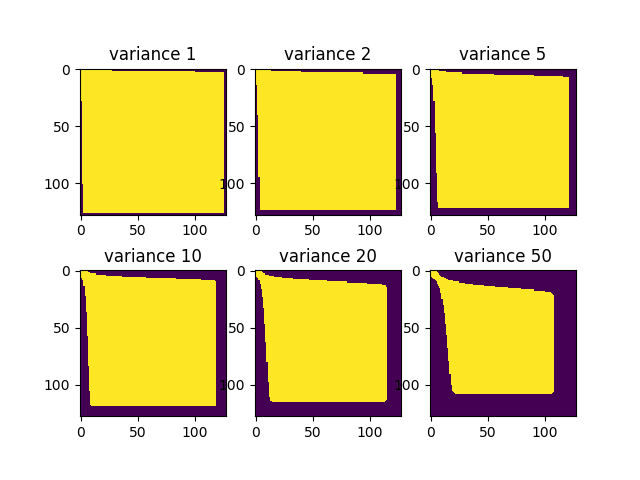
\includegraphics[width=0.7\textwidth]{softargmax_variance_test.png}
    \caption{Evaluation of the accuracy of the Soft-argmax function using synthetic data. Yellow pixels $i,j$ indicate where the Soft-argmax function correctly regressed the peak of the gaussian with mean value $i,j$, while violett indicates wrong predictions. Notice that the accuracy decreases when approaching the border of the image and when the covariance is increasing. }
    \label{fig:softargmax_variance_test}
\end{figure}

\subsection{Replication of Original Work}
\label{sec:exp-replication}

\subsubsection{Pose estimation}

\subsubsection{HAR using Penn Action dataset}

\subsection{Pose estimation on JHMDB dataset}

\subsection{HAR using on JHMDB Dataset}
all kinds of substitutions like using gt bb etc.

\subsection{Effect of Combining Loss Functions}
e2e

\subsection{Effect of Using Different Representations of Pose}
\label{sec:different_pose_representation_experiment}

